\usepackage{booktabs}
\usepackage[nottoc,numbib]{tocbibind}
\usepackage{amsmath}
\usepackage{color}
\usepackage{amsbsy}
\usepackage[normalem]{ulem}
\usepackage{cancel}
\usepackage[svgnames]{xcolor}
\usepackage{framed}
%\colorlet{shadecolor}{Silver} Probably too dark...
\colorlet{shadecolor}{WhiteSmoke}
\colorlet{framecolor}{Silver}
\usepackage{float}
\usepackage{caption}
\newgeometry{inner=1.25in,outer=0.75in,top=1in,bottom=1in}

\definecolor{purple}{RGB}{76,0,153}

% % make code-output smaller
% \DefineVerbatimEnvironment{Highlighting}{Verbatim}{fontsize=\tiny,commandchars=\\\{\}}
% 

% make console-output smaller:
%  \makeatletter
% \def\verbatim{\small\@verbatim \frenchspacing\@vobeyspaces \@xverbatim}
% \makeatother

\setlength{\parindent}{15pt} % Default is 0pt.

%\setlength{\parskip}{0pt}


\setlength{\OuterFrameSep}{0pt}
\setlength{\FrameRule}{1.5pt}
\makeatletter
\def\preto{\@verbatim}{\topsep=-10pt \partopsep=-10pt }
\makeatother

% Adjust verbatim shade environments

\renewenvironment{Shaded}{%
\setlength{\FrameRule}{1.5pt}
\def\FrameCommand{\fboxrule=\FrameRule\fboxsep=\FrameSep \fcolorbox{framecolor}{shadecolor}}%
\MakeFramed {\FrameRestore}}%
{\endMakeFramed}



%Change third level of itemize to an open circle instead of an asterisk
\renewcommand{\labelitemiii}{$\circ$}

\newcommand{\BD}{\boldsymbol{\Delta}}

\renewcommand*{\maketitle}{%
\begin{titlepage}
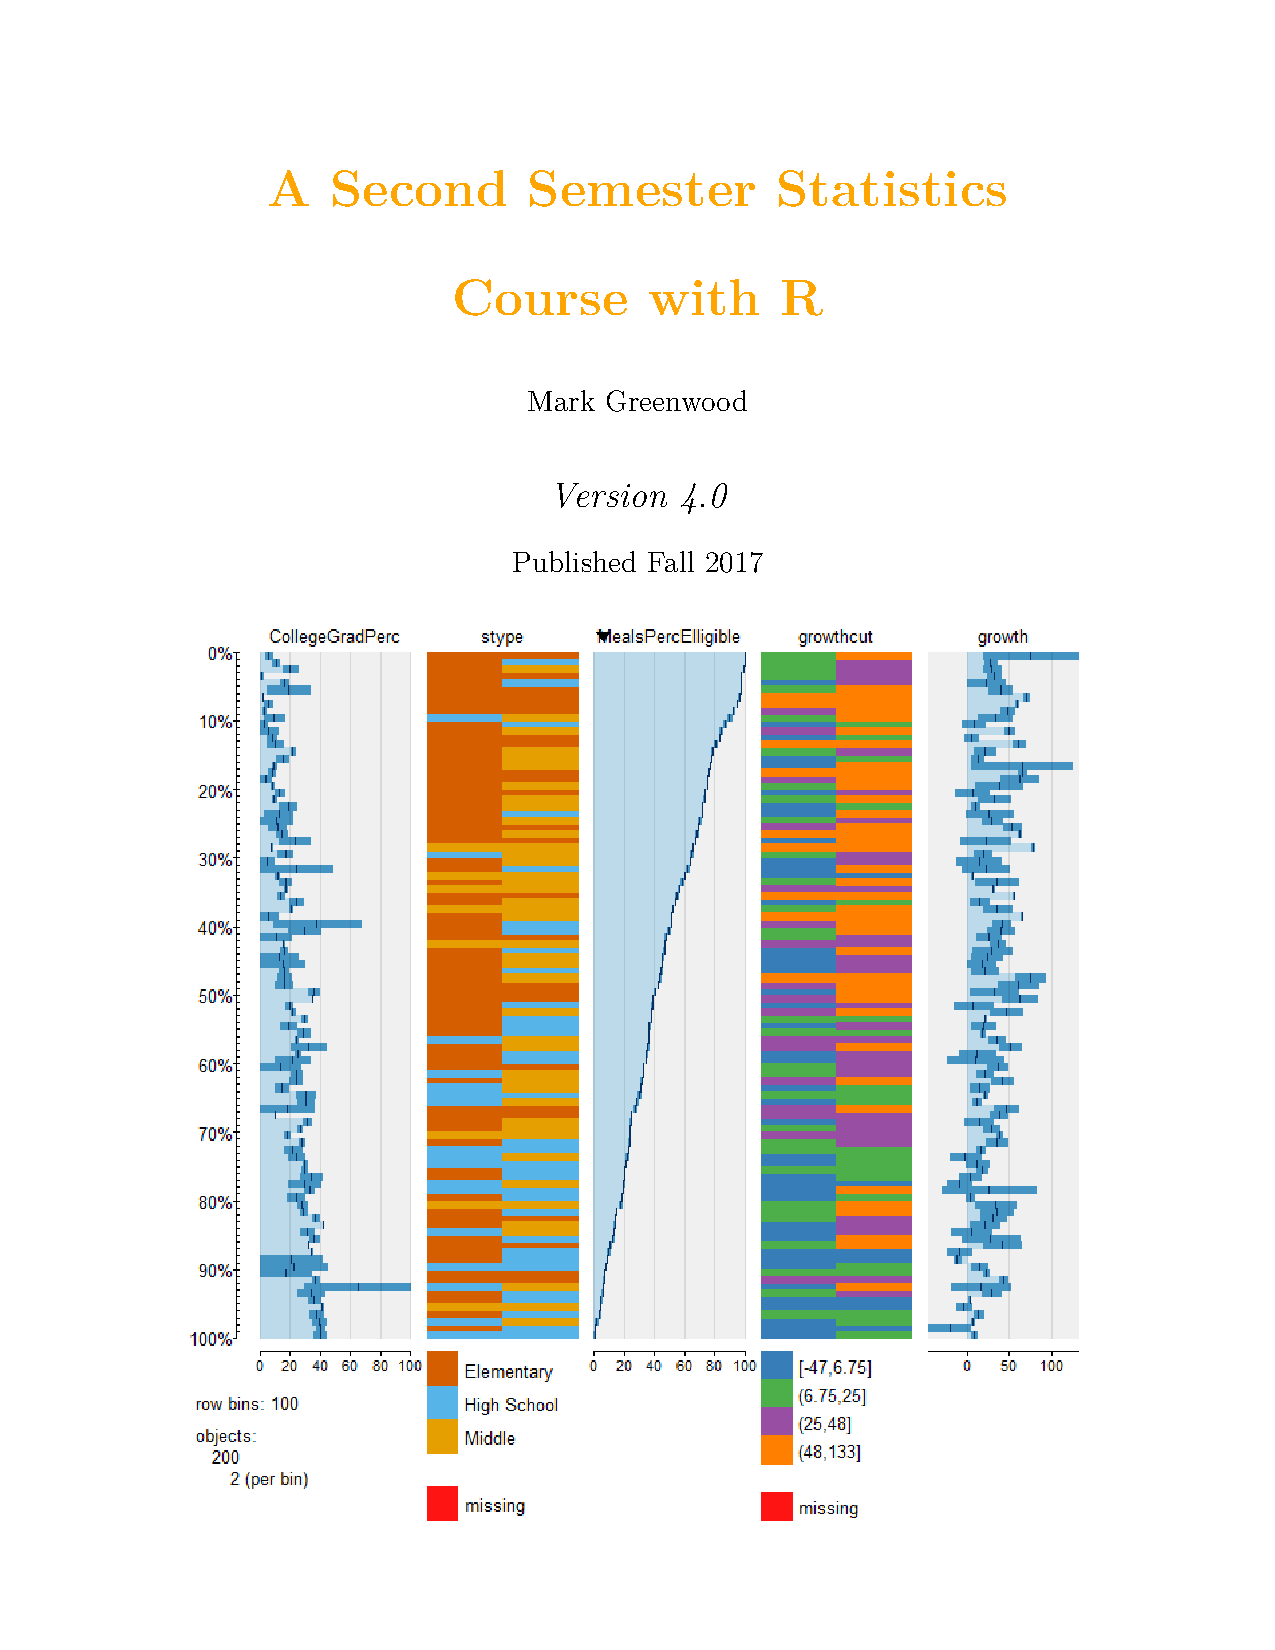
\includegraphics{titlepage.pdf}
\end{titlepage}
}
